\chapter{\label{ch:6}Regulation of Kir6.2 by SUR1} 

\graphicspath{{figures/tempfigs/}}

\minitoc

\section{Introduction}
The SUR1 subunit exerts a number of different regulatory effects on the K\ATP{} channel.
Firstly, it dramatically enhances trafficking of Kir6.2 to the cell membrane by masking the endoplasmic retention motif in Kir6.2 (RKR).
Without coexpression with SUR1, Kir6.2 is confined to the endoplasmic reticulum.
Truncating the C-terminal by deleting the last 26 (Kir6.2-\textgreek{D}C26) or 36 (Kir6.2-\textgreek{D}C36) amino acids \cite{tucker_truncation_1997}, mutation of the RKR motif to AAA \cite{zerangue_new_1999}, or addition of a C-terminal GFP tag \cite{john_sulphonylurea_1998} are sufficient to allow expression of Kir6.2 at the membrane alone without the presence of SUR1.
Comparing the function of these modified Kir6.2 subunits alone to the function of octameric K\ATP{} channels makes it possible to discern the multifaceted roles of SUR1.
Crucially, these C-terminal modifications do not appear to alter K\ATP{} function when they are coexpressed with SUR1 \cite{tucker_truncation_1997, john_sulphonylurea_1998, ribalet_atp-sensitive_2006} and the cryo-EM structure solved for C-terminally GFP labelled Kir6.2 \cite{li_structure_2017} was highly similar to those solved without the GFP label \cite{martin_anti-diabetic_2017-1, lee_molecular_2017-1}.

Coexpression of SUR1 has two effects on K\ATP{} channel function.
Firstly, SUR1 increases the $P_O$ of the channel \cite{tucker_truncation_1997, john_sulphonylurea_1998, chan_n-terminal_2003-1}.
Expressing the TMD0 region of SUR1 (residues 1 - 195) alone is sufficient to recapitulate the increase in $P_O$ observed when full-length SUR1 is coexpressed\cite{babenko_sur_2003-1, chan_n-terminal_2003-1}.
When TMD0 is coexpressed with Kir6.2, there is additionally a decrease in the sensitivity of Kir6.2 to nucleotide inhibition - allosterically, an increase in $P_O$ would result in a decrease in apparent ATP affinity due to the reduction in stability of the closed state.
However, when full length SUR1 is coexpressed with Kir6.2, there is a marked increase in sensitivity to ATP inhibition \cite{tucker_truncation_1997, john_sulphonylurea_1998, chan_n-terminal_2003-1, ribalet_atp-sensitive_2006}.
This increase in sensitivity is not due to the L0 linker, the other domain of SUR1 postulated to make contacts with Kir6.2.
Expression of TMD0-L0 (residues 1 - 232) with Kir6.2 increases the $P_O$ to nearly saturating, and reduces ATP inhibition even further \cite{babenko_sur_2003-1}.
Increasing the fraction of L0 (up to residue number 256 or 288) attenuates this increase in $P_O$, but there is not the dramatic increase in ATP sensitivity observed from expression of full-length SUR1, implicating a role for the core region of SUR1 in regulating nuclelotide binding and inhibition \cite{puljung_cryo-electron_2018}.

\section{Intrinsic effects of SUR1}

\subsection{SUR1 alters nucleotide inhibition, but not binding}
Expressing WT-GFP alone without SUR1 results in smaller, noisier currents than when coexpressed with SUR1.
Currents are less sensitive to ATP and TNP-ATP by an order of magnitude (x and x).
Our surface expression assay suggested that while WT-GFP was able to reach the membrane in the absence of SUR1, W311*-GFP was not, and when we excised patches from cells expressing W311*-GFP alone, we were not able to resolve any currents.
We were still able to resolved fluorescence in unroofed membranes expressing W311*-GFP alone, and so we measured binding of TNP-ATP to W311*-GFP alone in unroofed membranes.
We observed very minimal differences in the EC\textsubscript{50} for binding.
However, given that we did not observe currents under these experimental conditions, we cannot determine the functional state of these channels and so this finding may not be representative for K\ATP{} channels physiologically.

Given that we were able to observe currents in the absence of SUR1, we confirmed that when SUR1 was cotransfected with our constructs we were measuring currents and fluorescence from correctly assembled K\ATP{} channels.
Firstly, we used tolbutamide to inhibit excised patches from cells expressing either WT-GFP alone, WT-GFP+SUR1 or W311*-GFP+SUR1.
Tolbutamide inhibition occurs at two sites on the K\ATP{} channel; a high affinity site on SUR1 and a low affinity site on Kir6.2 \cite{gribble_tissue_1998, ashfield_identification_1999}.
Inhibition occurring at these two sites can be well separated, with the high affinity site saturating at \SI{100}{\micro\Molar} tolbutamide at \SI{50}{\percent} fractional inhibition.
Tolbutamide inhibition of Kir6.2 expressed alone does not display inhibition until concentrations of over \SI{100}{\micro\Molar}.
When we expressed WT-GFP alone, we saw no inhibition of currents by \SI{100}{\micro\Molar}, whereas when we expressed WT-GFP+SUR1 or W311*-GFP+SUR1, we observed roughly a \SI{50}{\percent} fractional inhibition of current as expected for proper associated of Kir6.2 and SUR1.

\begin{figure}[h]
	\centering
	\begin{subfigure}[t]{0.45\textwidth}
		\caption{}\label{ch6fig:nosur_patch}
		\centering
		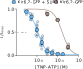
\includegraphics[width=\textwidth]{nosur_patch.pdf}
	\end{subfigure}
	\hfill
	\begin{subfigure}[t]{0.45\textwidth}
		\caption{}\label{ch6fig:tolb_inhibition_1}
		\centering
		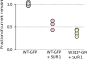
\includegraphics[width=\textwidth]{tolb_inhibition_1.pdf}
	\end{subfigure}
	\vfill
	\begin{subfigure}[t]{0.45\textwidth}
		\caption{}\label{ch6fig:nosur_unroofed}
		\centering
		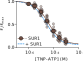
\includegraphics[width=\textwidth]{nosur_unroofed.pdf}
	\end{subfigure}
	\caption[SUR1 alters inhibition but not binding at Kir6.2]{
	}\label{ch6fig:no_sur}
\end{figure}

In addition, we labelled the C-terminus of SUR1 with the fluorophore mOrange (SUR1-mO), and measured FRET between the GFP on WT-GFP or W311*-GFP and the mOrange on SUR1 in unroofed membranes.
The cryo-EM structures suggest a distance between the C-termini of Kir6.2 and SUR1 of roughly \SI{60}{\angstrom}, while the GFP-mOrange FRET pair has a theoretical R0 of \SI{54}{\angstrom}.
We would therefore expect to see FRET if our Kir6.2 and SUR1 contructs are coassembling.
To measure FRET, we used an approach described in \cite{zheng_rod_2002} whereby FRET is measured as an increase in the emission of the acceptor fluorophore (mOrange) on excitation of the donor fluorophore (GFP) (Figure \ref{sur_assays}).
We observed FRET between WT-GFP and SUR1-mO, consistent with the two subunits being in close proximity.
Less FRET was observed when W311*-GFP was coexpressed with SUR1-mO (although still much higher than background).
This is probably due to the reduced expression of W311*-GFP compared to WT-GFP, i.e. there is less donor fluorescence to transfer to mOrange.
Correcting for the magnitude of the GFP peak results in observed ratios for WT-GFP and W311*-GFP that are very similar.

\begin{figure}[h]
	\centering
	\begin{subfigure}[t]{0.3\textwidth}
		\caption{}\label{ch6fig:gfp_mo_spectra_1}
		\centering
		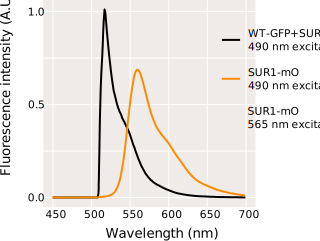
\includegraphics[width=\textwidth]{gfp_mo_spectra_1.pdf}
	\end{subfigure}
	\hfill
	\begin{subfigure}[t]{0.3\textwidth}
		\caption{}\label{ch6fig:wt_gfp_mo_spectra_1}
		\centering
		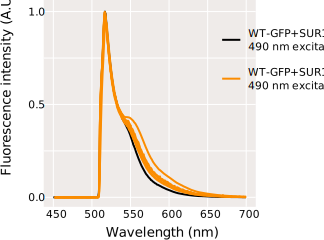
\includegraphics[width=\textwidth]{wt_gfp_mo_spectra_1.pdf}
	\end{subfigure}
	\hfill
	\begin{subfigure}[t]{0.3\textwidth}
		\caption{}\label{ch6fig:wt_gfp_mo_spectra_2}
		\centering
		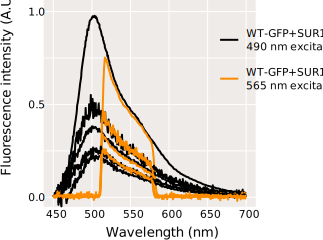
\includegraphics[width=\textwidth]{wt_gfp_mo_spectra_2.pdf}
	\end{subfigure}
	\vfill
	\begin{subfigure}[t]{0.3\textwidth}
		\caption{}\label{ch6fig:w311_gfp_mo_spectra_1}
		\centering
		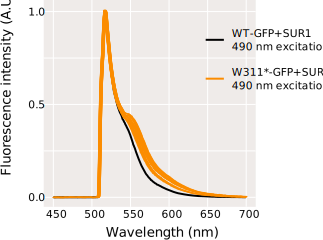
\includegraphics[width=\textwidth]{w311_gfp_mo_spectra_1.pdf}
	\end{subfigure}
	\hfill
	\begin{subfigure}[t]{0.3\textwidth}
		\caption{}\label{ch6fig:w311_gfp_mo_spectra_2}
		\centering
		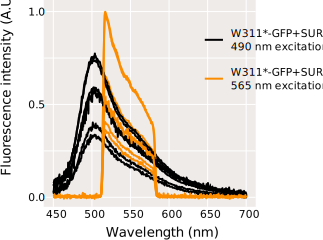
\includegraphics[width=\textwidth]{w311_gfp_mo_spectra_2.pdf}
	\end{subfigure}
	\hfill
	\begin{subfigure}[t]{0.3\textwidth}
		\caption{}\label{ch6fig:gfp_ofp_contrasts_1}
		\centering
		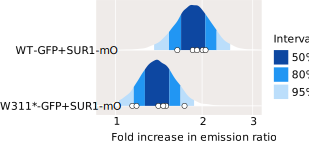
\includegraphics[width=\textwidth]{gfp_ofp_contrasts_1.pdf}
	\end{subfigure}
	\caption[SUR1 associates with WT-GFP and W311*-GFP]{
	}\label{ch6fig:sur_assays}
\end{figure}

\subsection{Presence of SUR1-TMD0 alone does not alter apparent nucleotide binding}

\begin{figure}[h]
	\centering
	\begin{subfigure}[t]{0.45\textwidth}
		\caption{}\label{ch6fig:tmd0s_surface_expression_1}
		\centering
		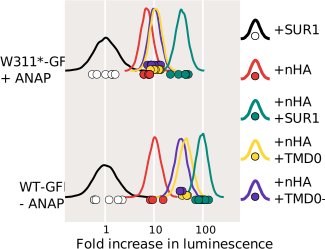
\includegraphics[width=\textwidth]{tmd0s_surface_expression_1.pdf}
	\end{subfigure}
	\hfill
	\begin{subfigure}[t]{0.45\textwidth}
		\caption{}\label{ch6fig:tmd0s_surface_expression_2}
		\centering
		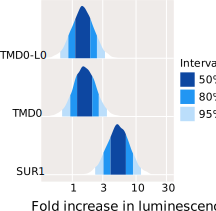
\includegraphics[width=\textwidth]{tmd0s_surface_expression_2.pdf}
	\end{subfigure}
	\vfill
	\begin{subfigure}[t]{0.45\textwidth}
		\caption{}\label{ch6fig:tmd0s_surface_expression_3}
		\centering
		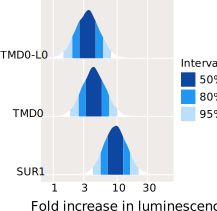
\includegraphics[width=\textwidth]{tmd0s_surface_expression_3.pdf}
	\end{subfigure}
	\hfill
	\begin{subfigure}[t]{0.45\textwidth}
		\caption{}\label{ch6fig:gfp_ofp_contrasts_2}
		\centering
		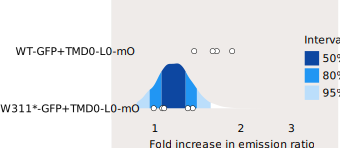
\includegraphics[width=\textwidth]{gfp_ofp_contrasts_2.pdf}
	\end{subfigure}
	\caption[TMD0 and TMD0-LO associate with WT-GFP and W311*-GFP]{
	}\label{ch6fig:tmd0_assays}
\end{figure}

\section{SUR1 and nucleotide regulation}

\subsection{Mutations at SUR-K205 alter nucleotide binding and inhibition}

\begin{figure}[h]
	\centering
	\begin{subfigure}[t]{0.45\textwidth}
		\caption{}\label{ch6fig:k205_1}
		\centering
		\includegraphics[width=\textwidth]{k205_1.pdf}
	\end{subfigure}
	\hfill
	\begin{subfigure}[t]{0.45\textwidth}
		\caption{}\label{ch6fig:k205_2}
		\centering
		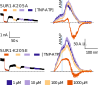
\includegraphics[width=\textwidth]{k205_2.pdf}
	\end{subfigure}
	\vfill
	\begin{subfigure}[t]{0.45\textwidth}
		\caption{}\label{ch6fig:mwc_k205_1}
		\centering
		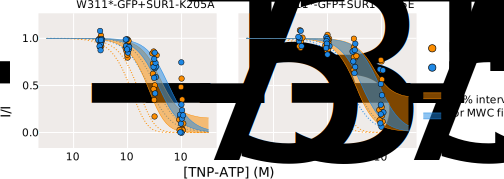
\includegraphics[width=\textwidth]{mwc_k205_1.pdf}
	\end{subfigure}
	\hfill
	\begin{subfigure}[t]{0.45\textwidth}
		\caption{}\label{ch6fig:mwc_k205_2}
		\centering
		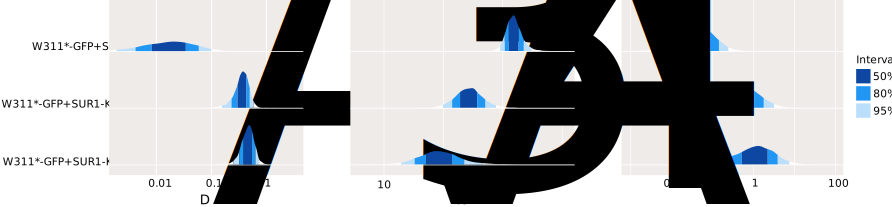
\includegraphics[width=\textwidth]{mwc_k205_2.pdf}
	\end{subfigure}
	\vfill
	\begin{subfigure}[t]{0.45\textwidth}
		\caption{}\label{ch6fig:mwc_k205_3}
		\centering
		
\includegraphics[width=\textwidth]{mwc_k205_3.pdf}
	\end{subfigure}
	\hfill
	\begin{subfigure}[t]{0.45\textwidth}
		\caption{}\label{ch6fig:mwc_k205_4}
		\centering
		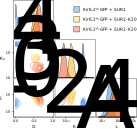
\includegraphics[width=\textwidth]{mwc_k205_4.pdf}
	\end{subfigure}
	\caption[SUR1 alteers inhibition but not binding]{
	}\label{ch6fig:no_sur}
\end{figure}

\subsection{The presence of magnesium does not affect nucleotide binding}

\section{Discussion}